\newpage
\begin{center}
	\textbf{\large 2. ПРАКТИЧЕСКАЯ ЧАСТЬ}
\end{center}
\refstepcounter{chapter}

\addcontentsline{toc}{chapter}{2. ПРАКТИЧЕСКАЯ ЧАСТЬ}

\section{Реализация оценочной функции}

Оценочная функция была реализована на языке программирования~С++ и~добавлена в~проект PSM в~виде набора модулей с~соответствующем разбиением на модуль интерфейса и~модуль реализации. Для нахождения взаимодействующих атомов был реализован алгоритм прямого перебора всех возможных пар атомов. 

Кратко процедура прямого перебора выглядит следующим следующим образом. Обрабатываются списки атомов хранящиеся в~ассоциативных контейнерах, где в~качестве ключа выступает идентификатор белковой цепи. При рассмотрении каждой пары атомов в~контейнере происходит сравнение расстояний между этими атомами и~формирование нового списка взаимодействующих атомов.

Очевидно, что в~случае, например, фиксированного количества атомов в~каждой цепи временная сложность такого алгоритма перебора возрастает со следующей асимптотикой: $O(n^2{\cdot}k{\cdot}(k-1)/2)$, где $k$ --~количество цепей, $n$ --~количество атомов в~одной цепи. В случае различного числа атомов в~цепях асимптотика прямого перебора также останется квадратичной.

Для ускорения процесса нахождения взаимодействующих пар атомов использовалась структура данных k-d-дерево. Оптимизированный алгоритм с~использованием k-d-дерева работает следующим образом. происходит перебор цепей ассоциативного контейнера и~строится соответствующее k-d-дерево. При этом требуется построение $k-1$ деревьев, где $k$ --~количество цепей в~комплексе. Сложность алгоритма $O(k^2 \cdot m \cdot build)$, где $k$ --~количество цепей, $n$ --~количество атомов в~цепи, по которой не построено k-d-дерево, $build = O(n \log_{2}{n})$ --~сложность постройки дерева. В общем случае, сложность поиска всех соседей в~k-d-дереве составляет $O(\log_{2}{n} + k)$, где $n$ --~количество точек в~дереве, а~k~--~количество найденных соседей в~заданном радиусе сферы взаимодействия атома. Также следует отметить, построенное k-d-дерево обладает фиксированной пространственной сложностью.

В случае отсутствия изменения в~позициях атомов некоторых компонентов комплекса нет необходимости строить дерево для каждой оценки. Например, в~случае если в~комплексе только два компонента и где только один меняет пространственную позицию достаточно построить дерево один раз для неподвижного компонента. В рамках исследования такой подход был реализован и обозначен как k-d-opt.


\section{Оптимизация с использованием k-d-дерева}


В данной работе для ускорения расчетов оценочной функции была реализована структура данных k-d-дерево на языке программирования C++ с поддержкой модулей. Поскольку библиотека PSM для полноатомного моделирования белка реализована на языке программирования C++ язык реализации оценочной функции и струткуры данных k-d-дерева идентичен.

Структура данных представляет собой отдельный подключаемый модуль в~рамках библиотеки и~представляет собой C++ структуру~KDTree, которая хранит в~себе указатель на корневой узел дерева и~содержит соответствующие методы для построения и~поиска взаимодействующих атомов. Листинг кода представлен в~Приложении~A.

% Про данные рассказано в первой главе
%\section{Платформа и тестовые данные для численных экспериментов}
%\section{Платформа для численных экспериментов}




\section{Результаты численных экспериментов}

Выполнение оценок разработанной оценочной функцией возможно только для полноатомных структур, представленных в~формате PDB. Поскольку оценочная функция разрабатывалась для моделирования процесса образования комплекса кинетическим методом Монте-Карло, для проверки качества выполняемых оценок был сформирован набор тестовых комплексов, взятый из хранилища SKEMPI~\cite{skempi}, представленный в работах~\cite{biom10071056, rate}. При этом из общего списка комплексов был выделен ограниченный набор структур. Исключены комплексы, содержащие разрывы в~главных цепях, а~также комплексы, состоящие из трёх и~более цепей. 

Перед проведением численного эксперимента для всех комплексов проведена предварительная подготовка. С~помощью пакета~CHARMM выполнено восстановление структур в полноатомный вид, поскольку представленные в~базе данных~PDB структуры могут не включать определенные атомы. Затем средствами пакета CHARMM выполнена минимизация энергии. В~результате для каждого комплекса формируются три стартовых PDB файла, для которых генерируются~PQR файлы, содержащие частичные заряды для каждого атома. На последнем этапе производится оценка энергии средствами~CHARMM и~разработанной оценочной функцией. Сформированный список комплексов и начальных файлов (PDB и~PQR) представлен в репозитории~\cite{vcs}.

Для проведения верификации оценочной функции использовался облачный сервис университета <<Дубна>>, в рамках которого использовался следующий процессор: Intel Xeon CPU E5-2650. Численные эксперименты, демонстрирующие применение k-d-дерева и~сравнение времени поиска взаимодействующих атомов другими инструментами, выполнено на процессоре AMD Ryzen 7 5700X на базовой частоте процессора равной 4.2 ГГц.

\subsection{Поиск взаимодействующих атомов}

На рис.~\ref{belki} представлено сравнение времени поиска взаимодействующих атомов для двух белков различными инструментами. 

Тестовый белковые комплексы 1TM1 и~1KXQ выбраны из библиотеки SKEMPI. Их различает разное число атомов. Второй комплекс содержит почти в~два раза больше атомов. Комплексы выбраны специально для объективности сравнения оценок при изменении числа атомов. Комплекс 1TM1 имеет два компонента (цепи), которые содержит 3939 и~1059 атомов соответственно. Комплекс 1KXQ также двухкомпонентный, каждая цепь содержит~7613 и~1786 атомов соответственно. Построение k-d-дерева во всех случаях происходило для первой цепи белкового комплекса.

Как видно из результатов, алгоритм с~применением прямого перебора всех атомов работает в~несколько раз медленнее других подходов. Однако, при сравнении с~Rosetta, несмотря на то, что коэффициент ускорения присутствует и~больше единицы, получаемое ускорение незначительно. Это связано с~тем, что в~Rosetta реализован собственный механизм построения карты взаимодействия атомов, который, в том числе, использует структуру данных k-d-дерево.

Обозначения на рисунках:
\vspace{-10pt}
\begin{enumerate}
	\setlength{\itemsep}{0pt}
	\setlength{\parskip}{0pt}	
	\item nn -- алгоритм прямого перебора всех атомов;
	\item rosetta -- программный комплекс Rosetta;
	\item k-d -- алгоритм с построением k-d-дерева при каждом поиске;
	\item k-d-opt -- алгоритм с предварительным построением k-d-дерева.
\end{enumerate}


\begin{figure}[h!]
	\captionsetup{justification=centering}
	\centering
	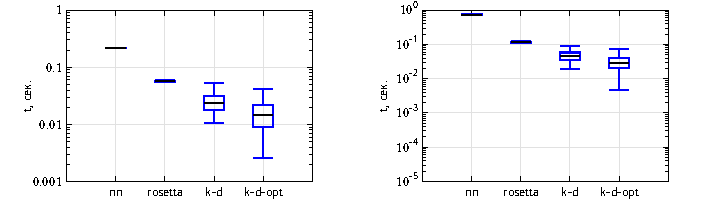
\includegraphics[width=1.0\linewidth]{images/bxpt.pdf}
	\caption{Время поиска взаимодействующих пар атомов для комплексов 1TM1 и 1KXQ}
	\label{belki}
\end{figure}

На рис.~\ref{acell} продемонстрированы коэффициенты ускорения соответствующие времени поиска взаимодействующих атомов разработанной функции в~отношении с другими алгоритмами. Всего выполнено 9154 оценки для белка 1TM1 и~9479 для комплекса 1KXQ. Следует отметить, что на представленных рисунках число контактов уникально и~не повторяется.

\begin{figure}[h!]
	\captionsetup{justification=centering}
	\centering
	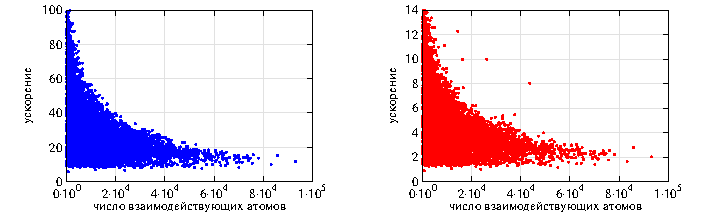
\includegraphics[width=1.0\linewidth]{images/accel.pdf}
	\caption{Получаемое ускорение при использовании алгоритма k-d-opt для комплекса 1KXQ \\ по сравнению с алгоритмом nn (слева) и Rosetta (справа)}
	\label{acell}
\end{figure}


\subsection{Верификация выполняемых оценок}


На рисунках~\ref{first} и~\ref{second} приведены результаты численных оценок для 84~комплексов. Средствами пакета CHARMM выполнена оценка энергии для представленных в~разработанной оценочной функции компонент. Для полученных значений рассчитан линейный коэффициент корреляции Пирсона.

Следует отметить, что представленная на рисунках оценка включает в~себя внутримолекулярные взаимодействия. Для этого в~оценочной функции и~в пакете CHARMM использовалась так называемая схема~1-3, где при формировании списка взаимодействующих пар атомов исключаются пары, которые связаны ковалентно~(схема~1-2), а~также пары, <<соединенные>> одним общим атомом. При рассмотрении компонент комплекса в~виде <<твёрдых>> тел внутримолекулярные взаимодействия изменяться не будут, поэтому при моделировании процесса образования комплекса достаточно выполнить их оценку только один раз и~затем рассматривать взаимодействия только между атомами компонент комплекса.

\begin{figure}[h!]
	\captionsetup{justification=centering}
	\centering
	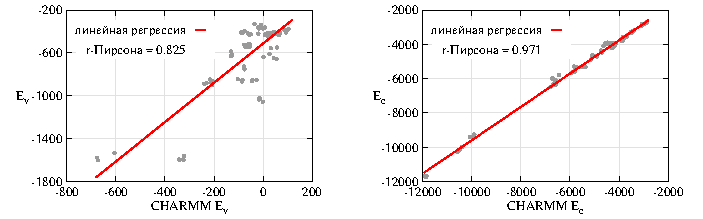
\includegraphics[width=1.0\linewidth]{images/first.pdf}
	\caption{Результаты численного эксперимента для потенциала Леннард-Джонса \\ и для потенциала Кулона}
	\label{first}
\end{figure}

\begin{figure}[h!]
	\captionsetup{justification=centering}
	\centering
	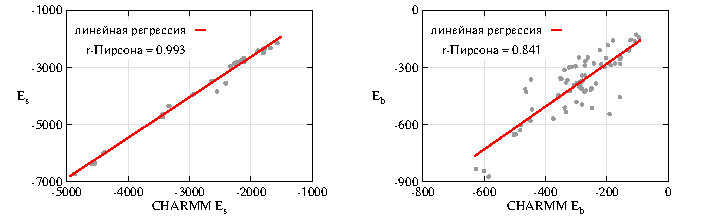
\includegraphics[width=1.0\linewidth]{images/second.pdf}
	\caption{Результаты численного эксперимента для неявного растворителя \\ и для оценки энергии связывания}
	\label{second}
\end{figure}

В простейшем случае процесс связывания описывается моделью вида ключ-замок, которая представляется в~виде $A+B\leftrightarrow AB$, где $A$ и~$B$ являются компонентами комплекса. С~помощью разработанной целевой функции возможно оценить энергию этого взаимодействия. На рисунке~\ref{second} продемонстрирована оценка энергии связывания без учета растворителя, которая определяется по следующей формуле:
\begin{equation}
	E_{b}=\left[E_{v}^{AB} + E_{c}^{AB}\right] - \left[E_{v}^{A} + E_{c}^{A} + E_{v}^{B} + E_{c}^{B}\right].
	\label{bind}
\end{equation}

В численном эксперименте в начальном PDB файле представлен образованный комплекс $AB$. При определении энергии связывания \eqref{bind} вычисляется разница между оценкой энергии комплекса в связанном состоянии и оценками энергий в свободном состоянии для каждого компонента в отдельности. В данном случае оценка энергии растворителя исключена для сравнения результатов оценки взаимодействия только на основе двух слагаемых оценочной функции.

На рис.~\ref{third} для тестового набора белков продемонстрировано сравнение оценок энергии связывания, которые были вычислены с~помощью разработанной оценочной функции (обозначено $F_s$). Для наглядности посчитана линейная регрессия и~коэффициент корреляции Пирсона.

В отличии от оценки $E_{b}$, слагаемые которой представлена в выражении~\ref{bind}, полная энергия связывания включает в~себя все три компонента (включая растворитель) и~вычисляется как разница между оценкой энергии комплекса в~связанном состоянии и~оценками энергий в~свободном состоянии, т.е.~когда компоненты комплекса друг с~другом не взаимодействуют. Представленная на рис.~\ref{third} оценка энергии связывания $\text{F}_{\text{s}}$ определяется следующим образом:

\begin{equation}
	\text{F}_{\text{s}}=F_{s}^{AB} - \left[F_{s}^{A} + F_{s}^{B}\right],
	\label{binde}
\end{equation}
где $F_{s}^{AB}$, $F_{s}^{A}$ и $F_{s}^{B}$ найденные с~помощью разработанной оценочной функции~\ref{totalf} значения.

\begin{figure}[h!]
	\captionsetup{justification=centering}
	\centering
	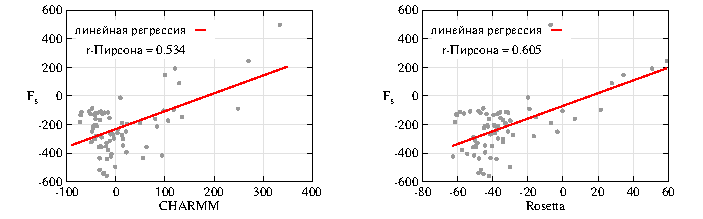
\includegraphics[width=1.0\linewidth]{images/third.pdf}
	\caption{Сравнение оценок энергии связывания разработанной оценочной функции \\ и оценок~вычисленных с~помощью других инструментов}
	\label{third}
\end{figure}
